\section{The OAL Framework for Mission Trust}

The \OAL{} framework provides a three-dimensional structure for classification and design. It can be used to locate a published mechanism, specify an assurance requirement, or identify an unprotected transition. The object dimension identifies \emph{what is judged}; the assurance dimension identifies \emph{which claim is sought}; and the lifecycle dimension identifies \emph{when the claim is needed}. These axes are conceptually distinct; evidence and failures across their cells can be dependent. A mechanism may occupy several cells, and some object--claim combinations are inapplicable to a particular mission. The framework organizes an assurance case by locating applicable claims; completeness and effectiveness require evidence about the relevant dependencies and outcomes. Figure~\ref{fig:oal} presents the framework.

\begin{figure}[!htbp]
\centering
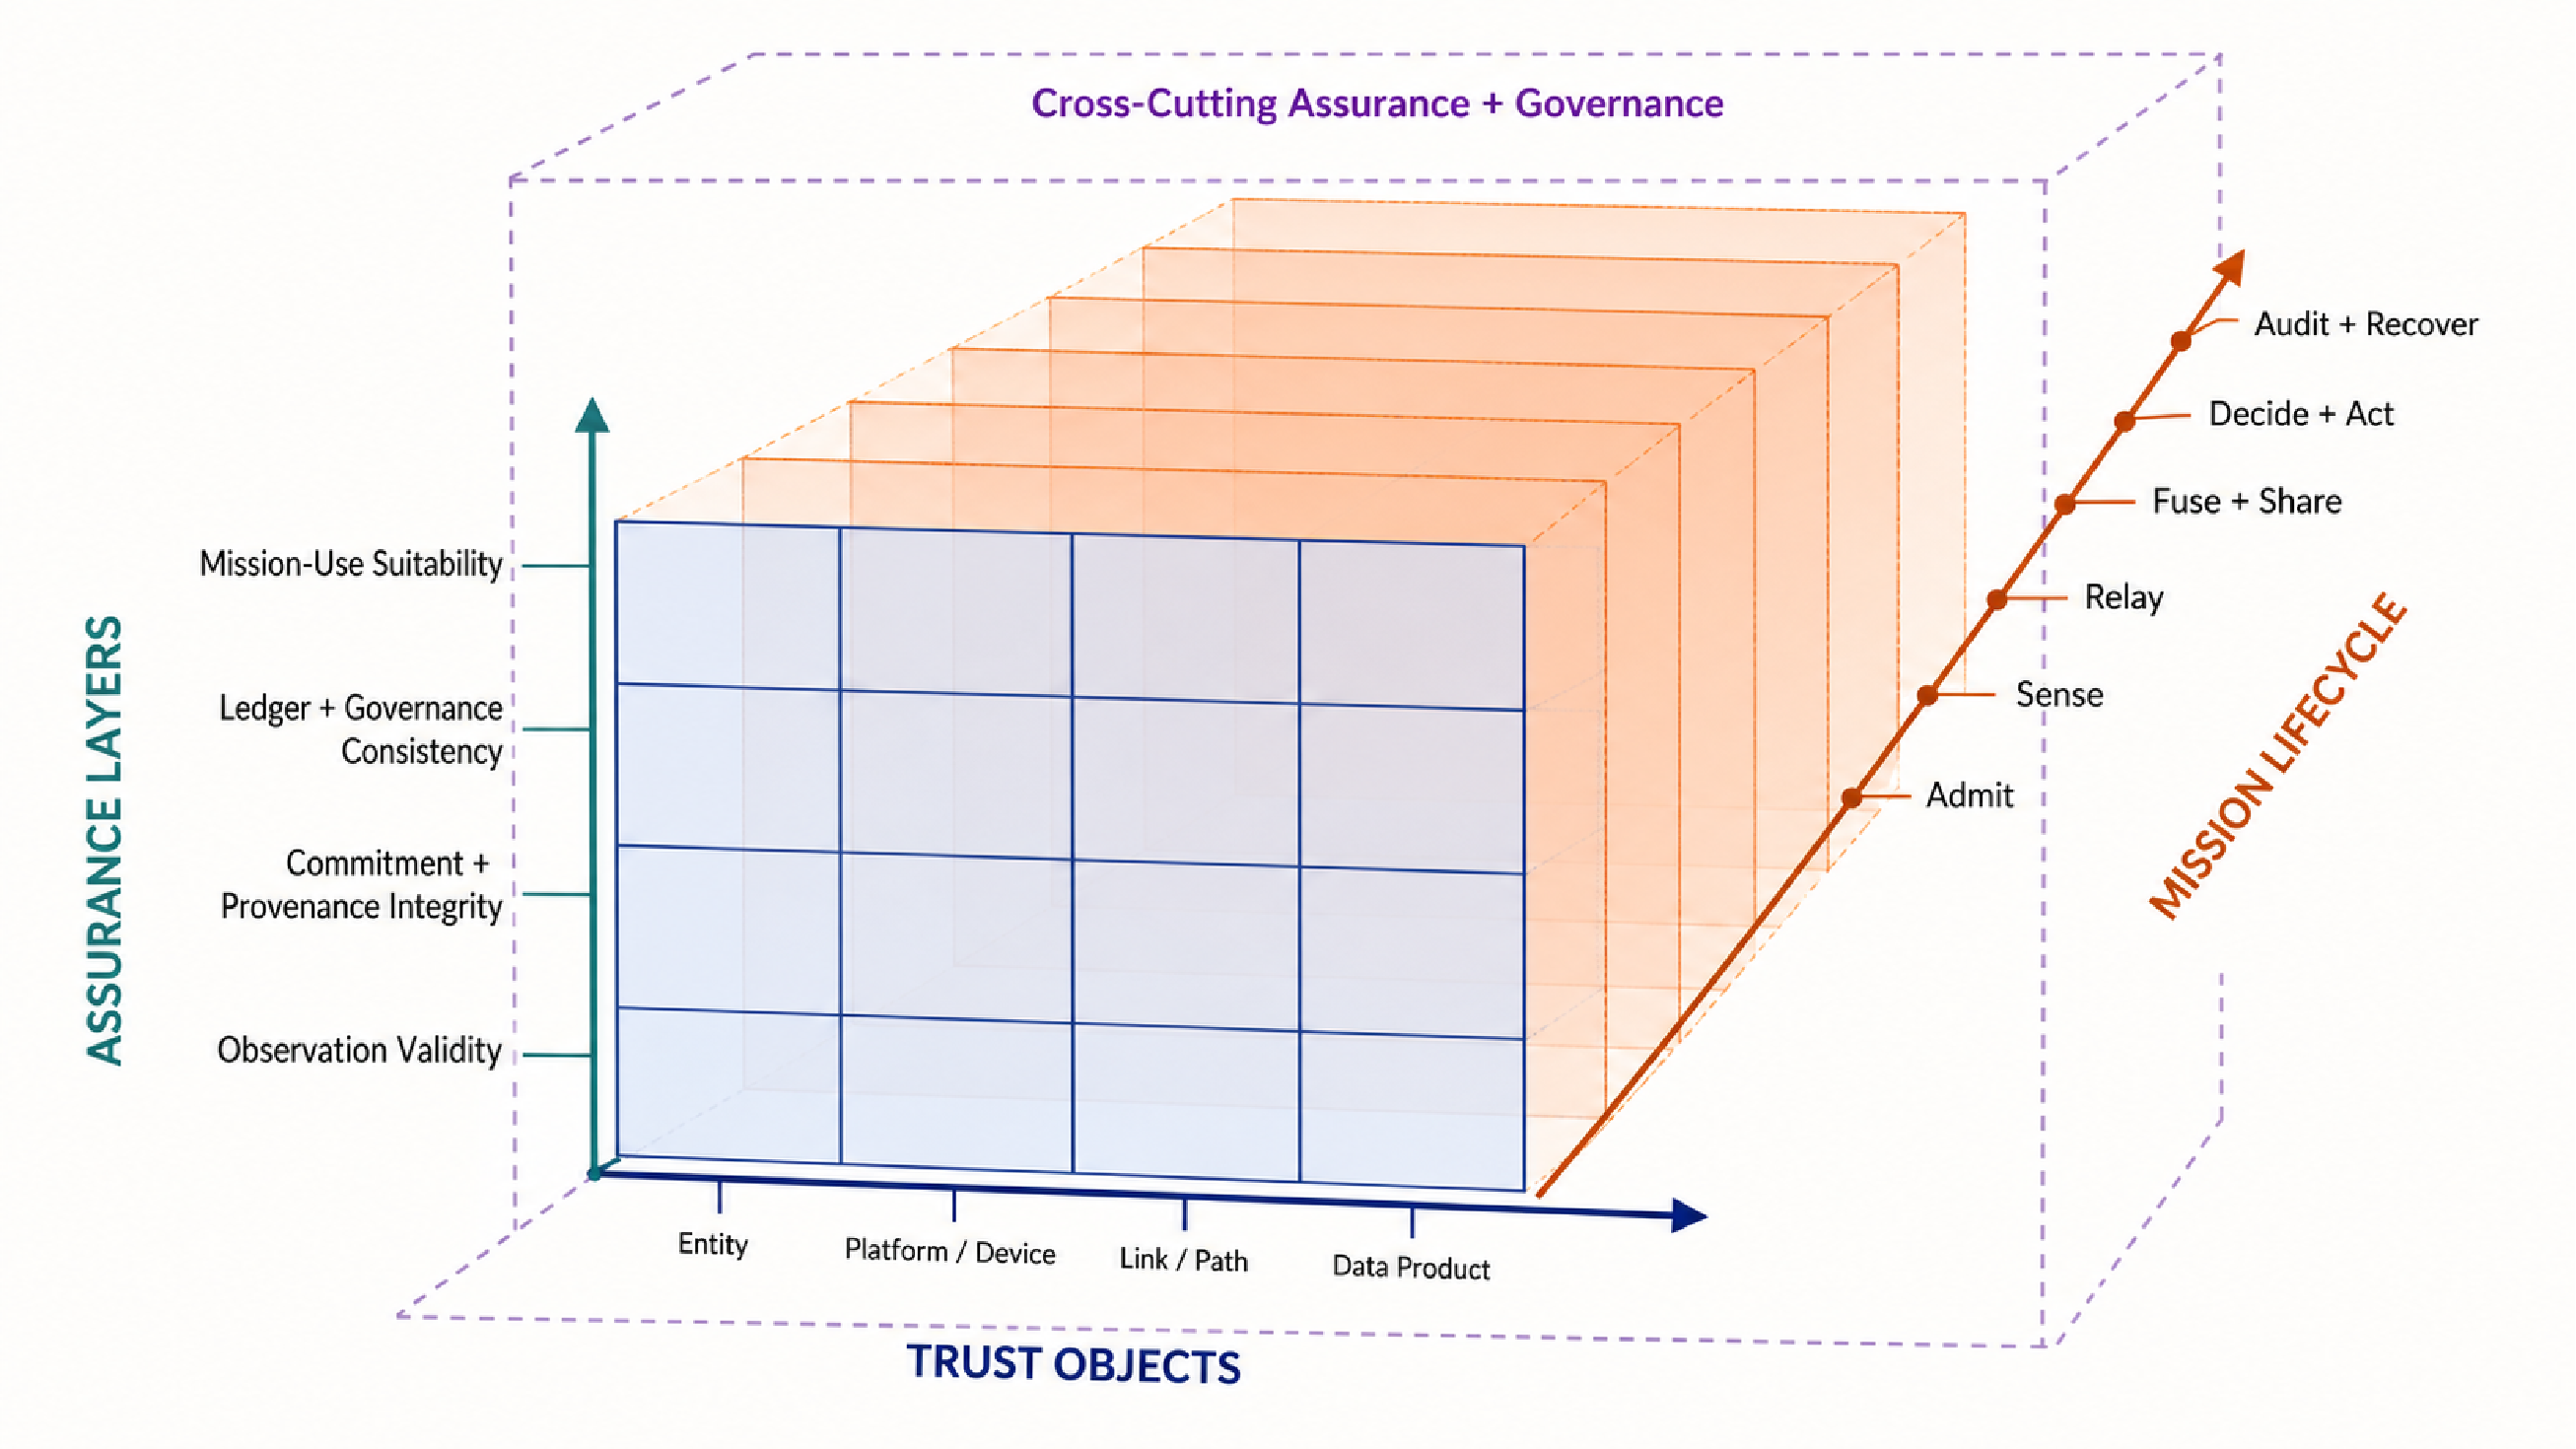
\includegraphics[width=\textwidth]{figures/figure-03-oal-framework.pdf}
\caption{OAL framework for mission trust. Trust objects run along the horizontal front-face axis, assurance layers along the vertical axis, and lifecycle stages along the oblique depth axis. Cells distinguish claims and their timing; the cross-cutting assurance and governance plane supplies shared services and dependencies.\label{fig:oal}}
\end{figure}

\subsection{Dimension I: Four Trust Objects}

An \emph{entity} is a principal capable of holding authority or responsibility: an operator, organization, mission service, software agent, or autonomous decision-making principal. A \emph{platform/device} is an executing physical or virtual endpoint: vehicle, sensor, gateway, compute module, secure element, or hosted execution instance. A stored software image or model artifact is a data product; its deployed state is assessed on the hosting endpoint. This distinction matters because an authorized entity can control a compromised device, while a device with valid attestation can execute a legitimate but unsuitable policy. An autonomous vehicle may occupy both categories under different claims: as a delegated principal for action and as an endpoint whose hardware and software state are measured.

A \emph{link/path} is a time-varying end-to-end route composed of its physical media, intermediate nodes, security associations, and quality state. A data product may traverse a UUV acoustic hop, a USV gateway, a satellite backhaul, and a cloud broker; confidentiality, freshness, availability, and routing integrity depend on this composed path. A \emph{data product} is an identified version of a raw observation, feature set, track, map, fused estimate, model output, command, alert, provenance record, or audit artifact. OAL treats a version as logically immutable: a transformation or correction creates a new identifier. This convention identifies versions; protection against storage alteration requires content verification and retained commitments.

\begin{table}[!htbp]
\caption{Four OAL trust objects, evidence, failure examples, and mission questions.\label{tab:objects}}
\begin{adjustwidth}{-\extralength}{0cm}
\small
\begin{tabularx}{\fulllength}{@{}P{25mm}YYY@{}}
\toprule
\textbf{Object} & \textbf{Representative evidence} & \textbf{Illustrative failure or attack} & \textbf{Mission question}\\
\midrule
Entity & Credential chain, organizational role, delegation, authorization, prior accountable actions & Credential theft, insider misuse, collusion, obsolete authority & Who requests, endorses, or consumes the resource, and under which authority?\\
Platform/device & Secure boot measurement, firmware/software version, sensor self-test, configuration, energy and health state & Capture, malware, unsafe configuration, stale reference value, sensor drift & Which endpoint executes, and is its measured state adequate for this use?\\
Link/path & Authentication state, route, delay, loss, signal indicators, neighbor changes, medium and gateway state & Jamming, wormhole, selective forwarding, eavesdropping, benign fading & Through which changing path did evidence pass, and what security and quality properties held?\\
Data product & Signature, timestamp, location, provenance graph, quality metadata, version, calibration and cross-source residuals & False injection, replay, poisoning, misregistration, unauthorized transformation & Where did this version come from, was it altered, and is it timely and suitable?\\
\bottomrule
\end{tabularx}
\end{adjustwidth}
\end{table}

Policies, models, smart contracts, and ledger state map onto the four operational object categories. They are versioned artifacts hosted on devices or represented as data products, while the principals who authorize them remain entities. This stable object set accommodates new mechanisms, and the assurance plane makes their artifacts first-class subjects of versioning, access control, threat analysis, and audit.

\subsection{Dimension II: Four Assurance Layers}

The first layer, \emph{observation validity}, asks whether evidence about the external world is credible. Relevant controls include calibration records, sensor diagnostics, geometry, physical bounds, environmental models, independent modalities, and temporal continuity. Multi-view and multi-sensor fusion can expose disagreement and express uncertainty \citep{holzinger2022information,liu2022trusted,qian2025review}; it can also amplify correlated error or poisoned inputs. Observation assurance therefore documents independence assumptions and combines physical and domain evidence with cryptographic content commitments.

The second layer, \emph{commitment and provenance integrity}, binds an item to recorded assertions about its producer, time, place, transformation, and version. Digital signatures, authenticated channels, secure timestamps, content identifiers, and W3C PROV relations support this layer \citep{w3c2013provdm,w3c2013provo,hu2020survey,pan2023data,singh2019decision}. A valid signature authenticates a statement under its key assumptions; the accuracy of the stated acquisition time or location requires separate evidence. Provenance covers both raw acquisition and model, human, or automated decisions. Decision provenance connects inputs, policy versions, intermediate transformations, and outputs, making later review possible when those records remain retrievable. Its assurance conditions include key custody, clock assumptions, instrumentation completeness, and trustworthy capture of events.

The third layer, \emph{ledger and governance consistency}, concerns shared state and the rules by which administrative parties maintain it. It covers member admission, endorsement, record ordering, validation, version coordination, revocation, dispute handling, and reconciliation. Hyperledger Fabric illustrates an execute--order--validate architecture with identity-aware channels and endorsement policies \citep{androulaki2018hyperledger,hyperledger2026fabric}; other shared-state services can satisfy the applicable functions. A ledger can establish agreement on validated records under a declared fault model. The legitimacy of governance rules, resolution of organizational disputes, and semantic validity of submissions require additional evidence and procedures. For missions using another shared-state architecture, the corresponding database or audit controls define the applicable assurance claims; ledger-specific claims are marked inapplicable.

The fourth layer, \emph{mission-use suitability}, applies a reliance policy to assurance evidence. Freshness, relevance, uncertainty, risk class, legal and organizational policy, available alternatives, and consequence severity are considered. A consumer may accept a low-resolution image for broad situational awareness but require corroborated, current, and accurately georegistered evidence for autonomous maneuver. An implementation assesses the required properties and separately applies the policy that permits, restricts, or defers an action. Authority to use the product requires the applicable authorization.

\subsection{Dimension III: Six Lifecycle Stages}

The lifecycle dimension prevents security from ending at admission. Table~\ref{tab:lifecycle} shows how objects and assurance questions evolve from credentialing to recovery. Evidence can age, dependencies can change, and an initially valid decision can require reassessment.

\begin{table}[!htbp]
\caption{Mission lifecycle and representative OAL assurance tasks.\label{tab:lifecycle}}
\begin{adjustwidth}{-\extralength}{0cm}
\small
\begin{tabularx}{\fulllength}{@{}P{30mm}YYP{38mm}@{}}
\toprule
\textbf{Stage} & \textbf{Primary questions} & \textbf{Evidence and controls} & \textbf{Ledger-relevant state}\\
\midrule
Admission and authentication & Is the entity authorized, and is the joining endpoint in an acceptable measured state? & Credentials, delegation, attestation, configuration baseline, least privilege & Membership, role, attestation-result commitment, policy version\\
Sensing and collection & Does an observation plausibly reflect its stated time, place, modality, and calibration? & Sensor self-test, secure time/location, quality metadata, corroboration & Acquisition commitment and data identifier\\
Transmission and relay & Which path carried the item, and did quality or security conditions change? & Mutual authentication, route and link telemetry, delay/loss context, custody transfer & Signed relay events or batch roots\\
Processing, fusion, and sharing & Which inputs, code, model, parameters, and policies produced this version? & Provenance graph, reproducible transformation identifier, access and usage control & Version, endorsement, access decision, model/policy commitment\\
Decision and action & Is the product fit for the specific mission consequence now? & Uncertainty, freshness, risk policy, alternatives, human review or fail-safe & Decision rationale commitment and responsible principal\\
Audit, revocation, and recovery & What failed, who was affected, what must be invalidated, and how is operation restored? & Incident evidence, credential and model revocation, rollback, re-attestation, after-action review & Revocation state, dispute outcome, reconciled log, recovery version\\
\bottomrule
\end{tabularx}
\end{adjustwidth}
\end{table}

Lifecycle continuity is especially difficult during partitions. During disconnection from a central policy engine, a UUV needs a local authorization envelope: named resources, permitted actions, risk limit, evidence freshness, expiry, and a context-appropriate fallback. Expiry enforcement requires bounded clock uncertainty and rollback-resistant local state, or a policy that reduces authority when those assumptions fail. Local actions are signed and sequenced; reconnecting nodes later disclose commitments and selected evidence. The design distinguishes \emph{continued operation under delegated authority} from \emph{fresh global authorization}; retained evidence supports later audit, while local enforcement constrains actions during disconnection.

\subsection{The Assurance and Governance Plane}

The cross-cutting plane contains identity and authorization, remote attestation, provenance capture, trust inference, policy/model/contract version management, ledger state, and consortium governance. Each component is itself attackable. Identity authorities can be compromised; reference values can be wrong; provenance instrumentation can omit transformations; a trust model can drift or be poisoned; a smart contract can encode an unsafe rule; validators can collude; and governance can deadlock. The plane must therefore be observed through the same OAL lens. For example, a model is a data product with provenance and validation evidence, a deployed instance is hosted on a device, its approval is an entity action, and its use is constrained by lifecycle stage and mission context.

OAL serves as both a diagnostic and a specification template. A blockchain-throughput study maps to ledger-performance cells and prompts complementary observation, endpoint, and mission-use requirements. A firmware-attestation protocol maps to a device claim at admission and prompts a freshness rule for disconnected decision time. For each applicable cell, a specification records the object/version, required property, evidence source and coverage, validity condition, acceptance rule, responsible party, and response to missing evidence. Reviewing identified high-consequence dependency paths then exposes absent or stale evidence. The resulting assurance case has the scope of its modeled paths; broader coverage requires identification and appraisal of additional dependencies.
